\documentclass[aspectratio=169]{beamer}


%%%%%%%%%%%%%%%%%%%%%%%%%%%%%%%%%%%%%%%%%%%%%%%%%%%%%%%%%%%%%%%%%%%%%%%%%%%%%%%%%
% PREAMBLE

% DEFINE VARIABLES
\newcommand{\Lesson}{TEMA EJEMPLO}
\newcommand{\Subject}{Ejemplos, ejemplos, y ejemplos}
\newcommand{\Program}{Inversiones Financieras}
\newcommand{\Professor}{CUNEF Universidad}

% FOOTER WITH LOGO
\setbeamertemplate{footline}{
\hfill
\includegraphics[width=1.2cm]{figs/logo.png}\hspace{13cm}\vspace*{0.5cm}
\insertframenumber \hspace{1cm}
}

% FOOTER WITHOUT LOGO
\newcommand{\NoLogoFootline}{
    \setbeamertemplate{footline}{
    \hfill\vspace*{0.5cm}    
    }
}

% PACKAGES
\usepackage{framed, color}
\definecolor{shadecolor}{rgb}{1,0.9,0.8}
\usepackage[absolute,overlay]{textpos}
\usepackage{graphicx, tikz,xcolor}
\usepackage{multirow, bigstrut,epstopdf}
\usepackage{amsmath,relsize,bigdelim}
\usepackage{hyperref}
\hypersetup{
    colorlinks=true,
    linkcolor=blue,
    filecolor=magenta,      
    urlcolor=cyan,
}
\usepackage[font=tiny]{caption}

\setbeamercolor{block body}{bg=CUNEFGray!20,fg=Front}
\setbeamercolor{block title}{bg=CUNEFOrange,fg=white}

\usetikzlibrary{shapes.geometric, arrows.meta}


% IDENTATION OPTIONS
\setlength{\leftmargini}{1em} % for itemize and enumerate level 1
\setlength{\leftmarginii}{1em} % for itemize and enumerate level 2
\setlength{\leftmarginiii}{1em} % for itemize and enumerate level 3

% COLOR OPTIONS
\definecolor{CUNEFOrange}{RGB}{255, 87, 0}
\definecolor{CUNEFGray}{RGB}{214, 209, 196}
\definecolor{Front}{RGB}{21,31,108}
% BEAMER OPTIONS
\setbeamertemplate{navigation symbols}{}
\setbeamercolor{itemize item}{fg = CUNEFOrange}
\setbeamercolor{itemize subitem}{fg = CUNEFOrange}
\setbeamercolor{itemize subsubitem}{fg = CUNEFOrange}		
\setbeamercolor{enumerate item}{fg = CUNEFOrange}
\setbeamercolor{enumerate subitem}{fg = CUNEFOrange}
\setbeamercolor{enumerate subsubitem}{fg = CUNEFOrange}		
\setbeamercolor{normal text}{fg=Front}

\setbeamercolor{frametitle}{fg=CUNEFOrange}

% NEW TITLE SLIDE
\newcommand{\CUNEFTitleSlide}{\begin{frame}



%\begin{textblock*}{0.1\paperwidth}(0.01\paperwidth,0.01\paperwidth)
%\includegraphics[width=0.3\paperwidth]{Logo_WQU.png}
%\end{textblock*}

\vspace{2em}
%\centering\scriptsize{{\textcolor{CUNEFOrange}{\Lesson}}} \\[1em]
\centering\textbf{{\large\textcolor{CUNEFOrange}{Econometrics 2024/2025}}} \\ [1em]
\centering{\large\textcolor{CUNEFOrange}{}} \\ [1em]
\vspace{0.5em}
\centering{\normalsize\textcolor{CUNEFOrange}{Topic 1: Simple Regression Model}}
\end{frame}}

% NEW SLIDE TEMPLATE
\newcommand{\slide}[2]{\begin{frame}
%\begin{textblock*}{0.1\paperwidth}(0.01\paperwidth,0.01\paperwidth)
%\includegraphics[width=0.15\paperwidth]{Logo_WQU.png}
%\end{textblock*}


\begin{textblock*}{0.87\paperwidth}(0.05\paperwidth,1.2cm)
{\Large\textcolor{CUNEFOrange}{#1}}
\end{textblock*}

\begin{textblock*}{0.87\paperwidth}(0.05\paperwidth,2cm)
#2
\end{textblock*}

\begin{textblock*}{\paperwidth}(0.01\paperwidth,0.95\paperheight)
\noindent\begin{tikzpicture}
%\draw[CUNEFOrange] (0,0) rectangle (0.9\paperwidth,0.8em);
%\draw[CUNEFOrange] (0.9\paperwidth+0.01\paperwidth,0) rectangle (\paperwidth-0.02\paperwidth,0.8em);
%\node[right] at (0,0.4em) {\tiny\textcolor{CUNEFGray}{\Subject\enspace-- \Program\enspace-- \Professor\enspace}};
\end{tikzpicture}
{\tiny\textcolor{CUNEFGray}\thepage}
\end{textblock*}
\end{frame}
}
%%%%%%%%%%%%%%%%%%%%%%%%%%%%%%%%%%%%%%%%%%%%%%%%%%%%%%%%%%%%%%%%%%%%%%%%%%%%%%%%%

% TOC AT BEGINNING OF EACH SECTION
\AtBeginSection[]{
    \begin{frame}<beamer>
    \frametitle{\textcolor{CUNEFOrange}{Outline}}
    \tableofcontents[currentsection]
    \end{frame}
}

\begin{document}

%%%%%%%%%%%%%%%%%%%%%
% Title Page
%%%%%%%%%%%%%%%%%%%%
\NoLogoFootline
{\usebackgroundtemplate{%
  
\includegraphics[width=\paperwidth,height=\paperheight]{figs/title_page.png}}
\CUNEFTitleSlide}

%%%%%%%%%%%%%%%%%%%%%
% Start slides
%%%%%%%%%%%%%%%%%%%%
\setbeamertemplate{footline}{
\hfill
\includegraphics[width=1.2cm]{figs/logo.png}\hspace{13cm}\vspace*{0.5cm}
\insertframenumber \hspace{1cm}
}

\begin{frame}
\frametitle{\textcolor{CUNEFOrange}{Outline}}
   \tableofcontents 
\end{frame}


\section{The simple regression model}
\frame<beamer>{\frametitle{\textcolor{CUNEFOrange}{The simple regression model}}
\begin{itemize}
\item We are often interested in ``explaining y in terms of x'', or in studying ``how y changes when x changes''. 

\item This can be achieved with the simple regression model.\medskip
\end{itemize}

%\begin{figure}
%    \centering
%    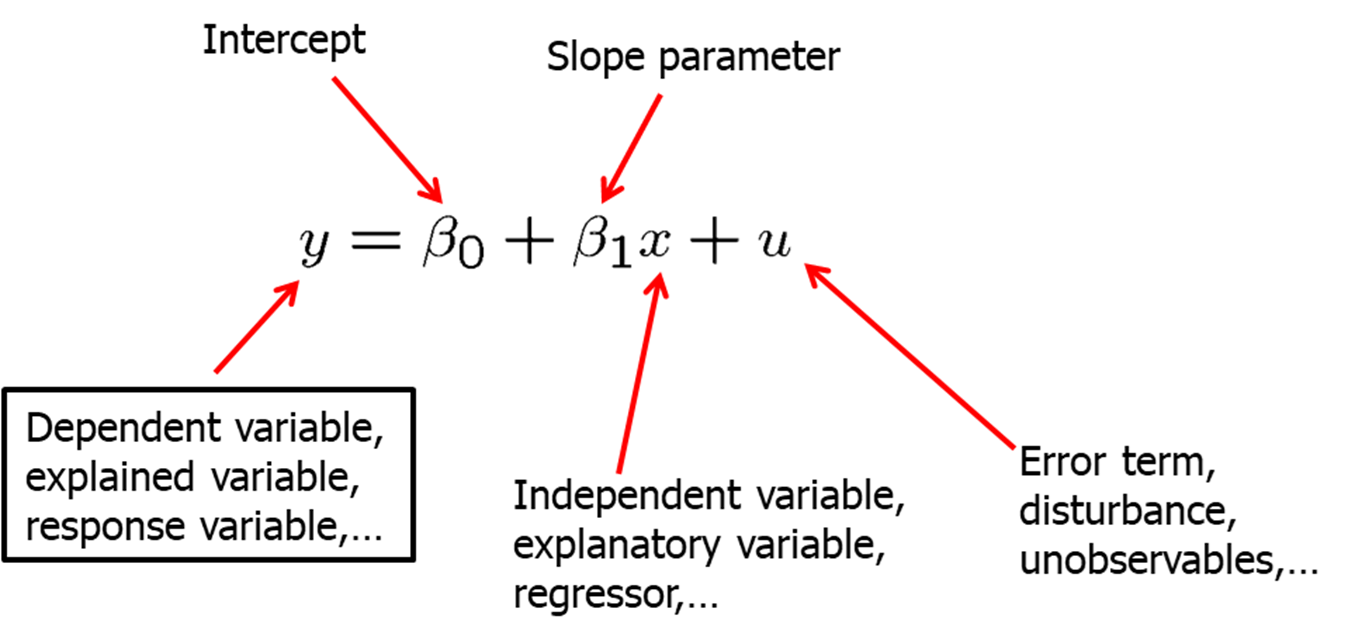
\includegraphics[width=0.8\linewidth]{figs/simple_reg.png}
%\end{figure}

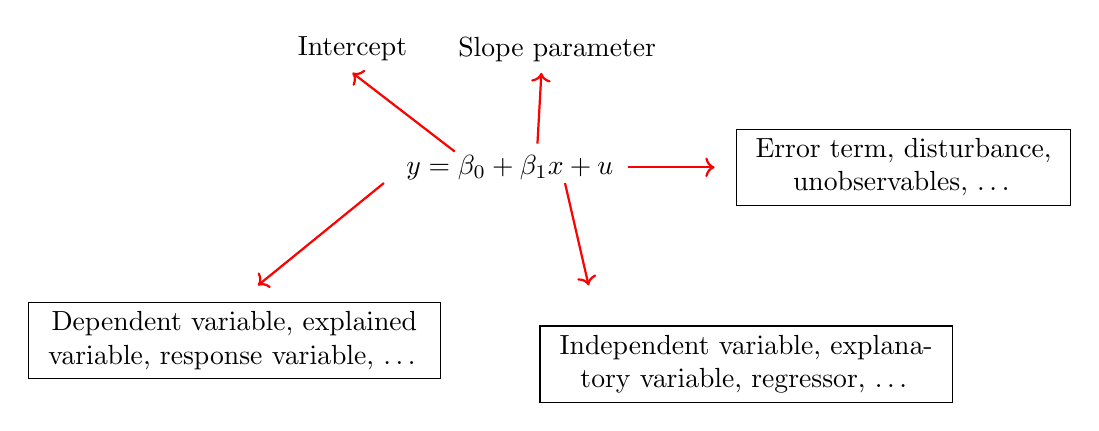
\begin{tikzpicture}

    % Equation
    \node at (0, 0) {\( y = \beta_0 + \beta_1 x + u \)};

    % Annotation for y (Dependent variable)
    \node[draw, rectangle, text width=5cm, align=center] at (-3.5, -2.2) {Dependent variable, explained variable, response variable, \dots};
    \draw[->, red, thick] (-1.6,-0.2) -- (-3.2,-1.5);

    % Annotation for beta_0 (Intercept)
    \node[align=center] at (-2, 1.5) {Intercept};
    \draw[->, red, thick] (-0.7, 0.2) -- (-2, 1.2);

    % Annotation for beta_1 (Slope parameter)
    \node[align=center] at (0.6, 1.5) {Slope parameter};
    \draw[->, red, thick] (0.35, 0.3) -- (0.4, 1.2);

    % Annotation for x (Independent variable)
    \node[draw, rectangle, text width=5cm, align=center] at (3, -2.5) {Independent variable, explanatory variable, regressor, \dots};
    \draw[->, red, thick] (0.7,-0.2) -- (1,-1.5);

    % Annotation for u (Error term)
    \node[draw, rectangle, text width=4cm, align=center] at (5, 0) {Error term, disturbance, unobservables, \dots};
    \draw[->, red, thick] (1.5, 0) -- (2.6,0);

\end{tikzpicture}


}

%%%%%%%%%%%%%%%%%%%%%%%%%%%%%

\frame<beamer>{\frametitle{\textcolor{CUNEFOrange}{ 
 The simple regression model}}

Interpretation of the simple linear regression model:\medskip

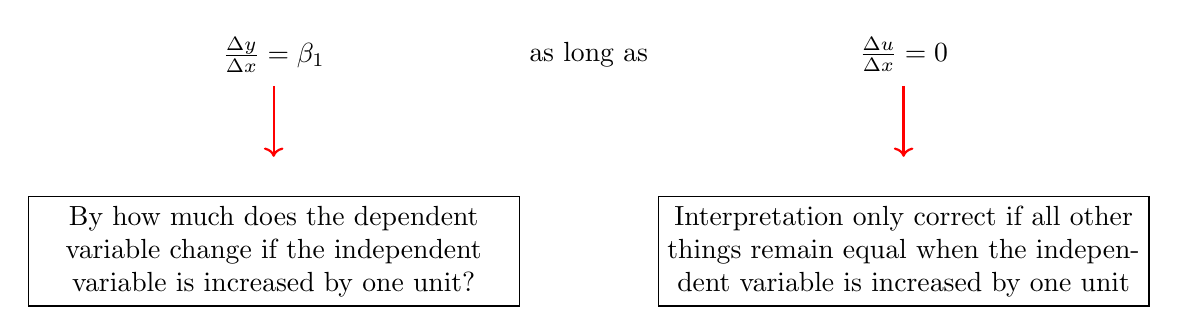
\begin{tikzpicture}

    % First equation
    \node at (0, 1) {$\frac{\Delta y}{\Delta x} = \beta_1$};

    % First box with annotation
    \node[draw, rectangle, text width=6cm, align=center] at (0, -1.5) {
        By how much does the dependent variable change if the independent variable is increased by one unit?
    };
    \draw[->, red, thick] (0,0.6) -- (0,-0.3);

    % As long as text
    \node at (4, 1) {as long as};

    % Second equation
    \node at (8, 1) {$\frac{\Delta u}{\Delta x} = 0$};

    % Second box with annotation
    \node[draw, rectangle, text width=6cm, align=center] at (8, -1.5) {
        Interpretation only correct if all other things remain equal when the independent variable is increased by one unit
    };
    \draw[->, red, thick] (8,0.6) -- (8,-0.3);

\end{tikzpicture}

}

%%%%%%%%%%%%%%%%%%%%%%%%%%%%%

\begin{frame}
\frametitle{\textcolor{CUNEFOrange}{The Simple Regression Model}}

\begin{itemize}
    \item \textbf{Example: CAPM equation}

    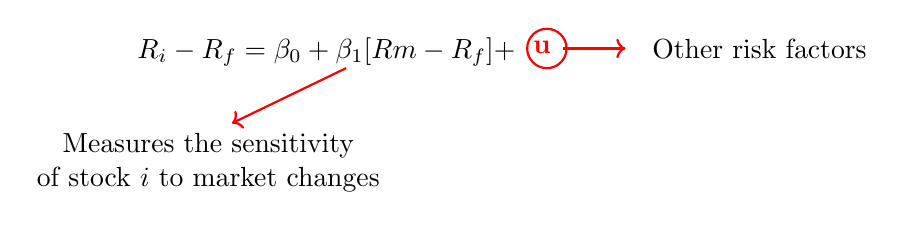
\begin{tikzpicture}

        % Equation
        \node at (0, 0) {$R_i - R_f = \beta_0 + \beta_1 [Rm-R_f] + $}; 

        % Circle around 'u' and annotation
        \node[anchor=west] at (2.5, 0.06) {\textcolor{red}{\textbf{u}}};
        \draw[red, thick] (2.8, 0.05) circle(0.25);

        % Annotation for beta_1
        \draw[->, red, thick] (0.25,-0.2) -- (-1.2,-0.9);
        \node[align=center] at (-1.5,-1.4) {Measures the sensitivity\\ of stock $i$ to market changes};

        % Annotation for u
        \draw[->, red, thick] (3, 0.05) -- (3.8, 0.05);
        \node[align=left] at (5.5, 0.05) {Other risk factors};

    \end{tikzpicture}

    \item \textbf{Example: wage equation}

    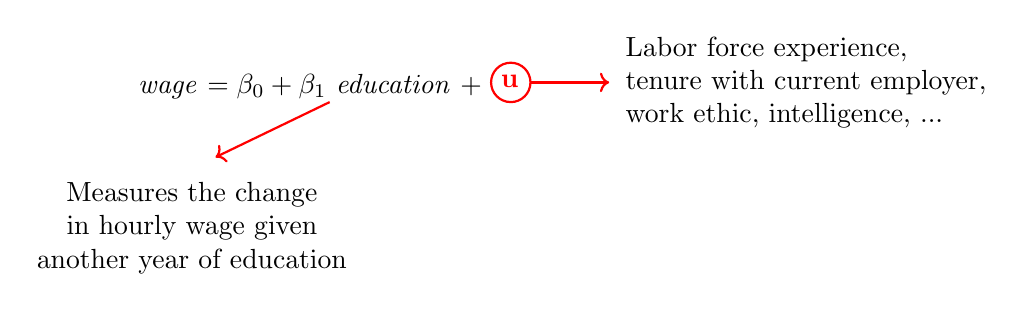
\begin{tikzpicture}

        % Equation
        \node at (0, 0) {\textit{wage} $= \beta_0 + \beta_1$ \textit{education} +};

        % Circle around 'u' and annotation
        \node[anchor=west] at (2.3, 0.06) {\textcolor{red}{\textbf{u}}};
        \draw[red, thick] (2.55, 0.05) circle(0.25);

        % Annotation for beta_1
        \draw[->, red, thick] (0.25,-0.2) -- (-1.2,-0.9);
        \node[align=center] at (-1.5,-1.8) {Measures the change\\ in hourly wage given\\ another year of education};

        % Annotation for u
        \draw[->, red, thick] (2.8, 0.05) -- (3.8, 0.05);
        \node[align=left] at (6.3, 0.05) {Labor force experience,\\tenure with current employer,\\ work ethic, intelligence, ...};

    \end{tikzpicture}

\end{itemize}

\end{frame}



%%%%%%%%%%%%%%%%%%%%%%%%%%%%%

\frame<beamer>{\frametitle{\textcolor{CUNEFOrange}{ 
 The simple regression model}}

\begin{itemize}
    \item Conditional mean independence assumption:
    $$
E(u \mid x)=0 
$$
\textbf{The explanatory variable must not contain information about the mean of the unobserved factors.}

    \item Example: wage equation

\begin{center}

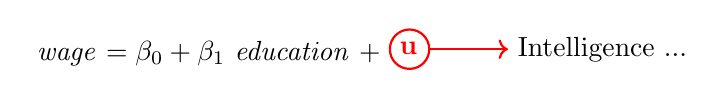
\begin{tikzpicture}

    % Equation
    \node at (0, 0) {\textit{wage} $= \beta_0 + \beta_1$ \textit{education} +};

    % Circle around 'u' and annotation
    \node[anchor=west] at (2.3, 0.06) {\textcolor{red}{\textbf{u}}};
    \draw[red, thick] (2.55, 0.05) circle(0.25);

  
    % Annotation for u
    \draw[->, red, thick] (2.8, 0.05) -- (3.8, 0.05);
    \node[align=left] at (5, 0.05) {Intelligence ...};

\end{tikzpicture}
    
\end{center}

The conditional mean independence assumption is unlikely to hold because individuals with more education will also be more intelligent on average.

\end{itemize}


}


%%%%%%%%%%%%%%%%%%%%%%%%%%%%%


\frame<beamer>{\frametitle{\textcolor{CUNEFOrange}{ 
The simple regression model}}

\textbf{Population regression function (PFR)}
\medskip
\begin{itemize}
    \item The conditional mean independence assumption implies that
    $$
\begin{aligned}
E(y \mid x) & =E\left(\beta_0+\beta_1 x+u \mid x\right) \\
& =\beta_0+\beta_1 x+E(u \mid x) \\
& =\beta_0+\beta_1 x
\end{aligned}
$$

\item  This means that the average value of the dependent variable can be expressed as a linear function of the explanatory variable.
\end{itemize}

}


%%%%%%%%%%%%%%%%%%%%%%%%%%%%%

\frame<beamer>{\frametitle{\textcolor{CUNEFOrange}{ 
The simple regression model }}

\begin{figure}
    \centering
    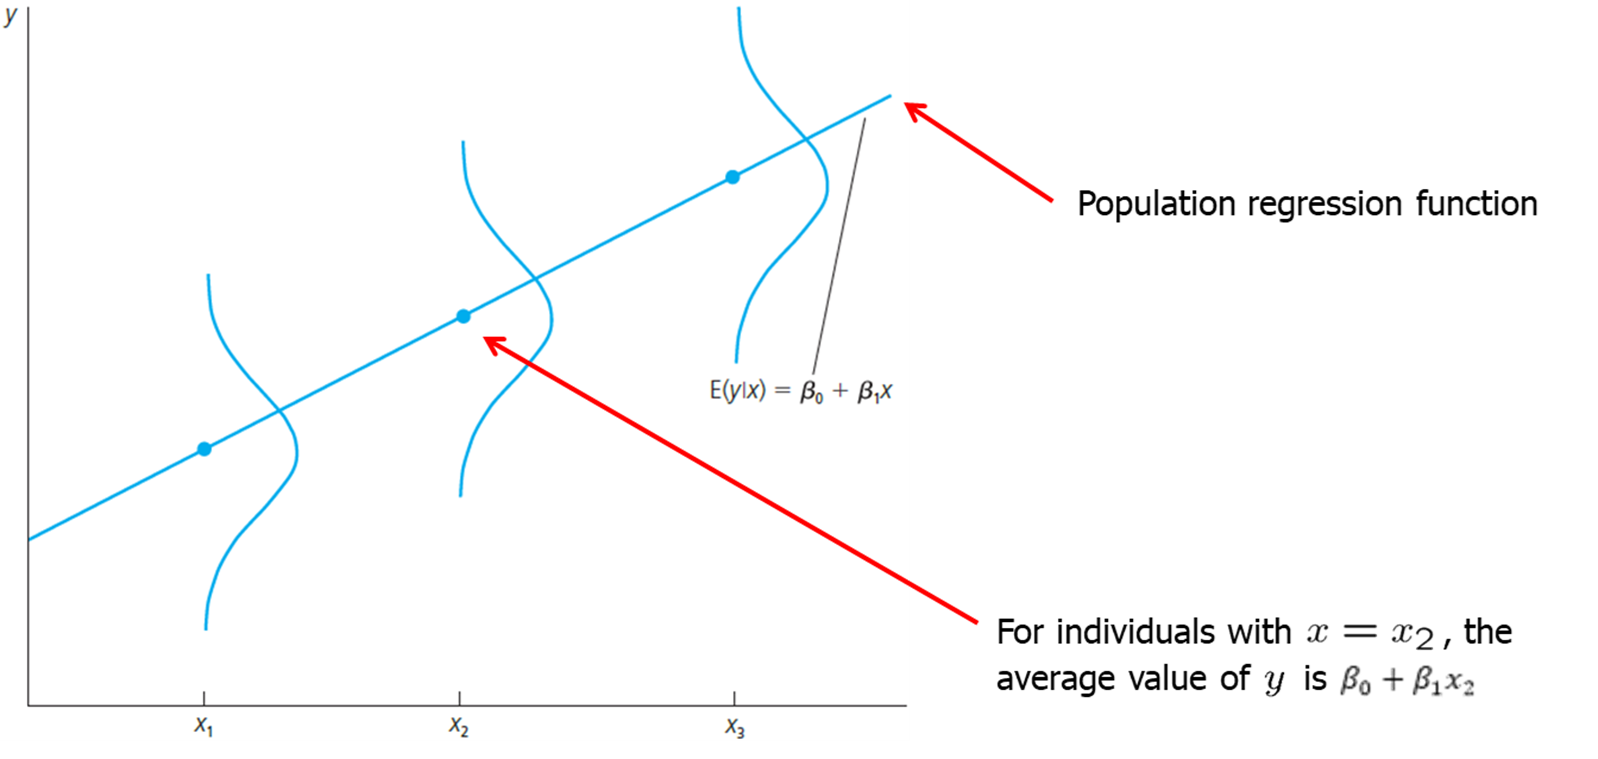
\includegraphics[width=1\linewidth]{figs/PRF.png}
\end{figure}
}

%%%%%%%%%%%%%%%%%%%%%%%%%%%%%
\section{Deriving the ordinary least squares (OLS) estimates}


\frame<beamer>{\frametitle{\textcolor{CUNEFOrange}{ 
Deriving the ordinary least squares (OLS) estimates
 }}

In order to estimate the regression model one needs random sample of $n$ observations

$$
\begin{gathered}
\left(x_1, y_1\right) \longleftarrow \text { First observation } \\
\,\,\,\,\,\left(x_2, y_2\right) \longleftarrow \text { Second observation } \\
\,\left(x_3, y_3\right) \longleftarrow \text { Third observation } \\
\vdots \\
\left(x_n, y_n\right) \longleftarrow \text { n-th observation }
\end{gathered}
$$
}

%%%%%%%%%%%%%%%%%%%%%%%%%%%%%

\frame<beamer>{\frametitle{\textcolor{CUNEFOrange}{ 
Deriving the ordinary least squares (OLS) estimates
 }}

\begin{itemize}
    \item Defining regression residuals
$$
\widehat{u}_i=y_i-\widehat{y}_i=y_i-\widehat{\beta}_0-\widehat{\beta}_1 x_i
$$
\item  Minimize the sum of the squared regression residuals (SSR)
$$
\min \text{SSR} = \min \sum_{i=1}^n \widehat{u}_i^2 \rightarrow \widehat{\beta}_0, \widehat{\beta}_1
$$
\item  OLS estimators
$$
\widehat{\beta}_1=\frac{\sum_{i=1}^n\left(x_i-\bar{x}\right)\left(y_i-\bar{y}\right)}{\sum_{i=1}^n\left(x_i-\bar{x}\right)^2}, \quad \widehat{\beta}_0=\bar{y}-\widehat{\beta}_1 \bar{x}
$$
\end{itemize}

}


%%%%%%%%%%%%%%%%%%%%%%%%%%%%%


\frame<beamer>{\frametitle{\textcolor{CUNEFOrange}{ 
Deriving the ordinary least squares estimates
 }}

\begin{itemize}
    \item Where do these expressions come from?

    \item Taking the first-order derivative of $\sum_{i=1}^n \widehat{u}_i^2$ with respect to $\beta_0$ and $\beta_1$ yields:
\[
\begin{array}{l}
 \frac{{\partial SSR}}{{\partial \beta _0 }} =  - 2\sum\limits_{i = 1}^n {\left( {y_i  - \beta _0  - \beta _1 x_i } \right) = 0}  \\
 \frac{{\partial SSR}}{{\partial \beta _1 }} =  - 2\sum\limits_{i = 1}^n {x_i \left( {y_i  - \beta _0  - \beta _1 x_i } \right) = 0}  \\
 \end{array}
\]

\item Algebraic manipulation of these two equations leads to the OLS expressions for $\widehat{\beta}_0$ and $\widehat{\beta}_1$.
    
\end{itemize}
}

\section{Properties of OLS}
%%%%%%%%%%%%%%%%%%%%%%%%%%%%%
\frame<beamer>{\frametitle{\textcolor{CUNEFOrange}{ 
Properties of OLS on any sample of data
 }}

\begin{itemize}
    \item Fitted (predicted) values 
$$
\widehat{y}_i=\widehat{\beta}_0+\widehat{\beta}_1 x_i 
$$

\item Residuals (deviations from the regression line)
$$
\widehat{u}_i=y_i-\widehat{y}_i
$$

    \item Deviations from regression line sum up to zero:    $$
\sum_{i=1}^n \widehat{u}_i=0
$$

\item Covariance between deviations and regressors is zero
$$
\sum_{i=1}^n x_i \widehat{u}_i=0
$$

\item Sample averages of $y$ and $x$ lie on regression line
$$
\bar{y}=\widehat{\beta}_0+\widehat{\beta}_1 \bar{x}
$$

\end{itemize}
}


%%%%%%%%%%%%%%%%%%%%%%%%%%%%%

\frame<beamer>{\frametitle{\textcolor{CUNEFOrange}{ 
OLS fits as good as possible a regression line through the data points
 }}

\begin{figure}
    \centering
    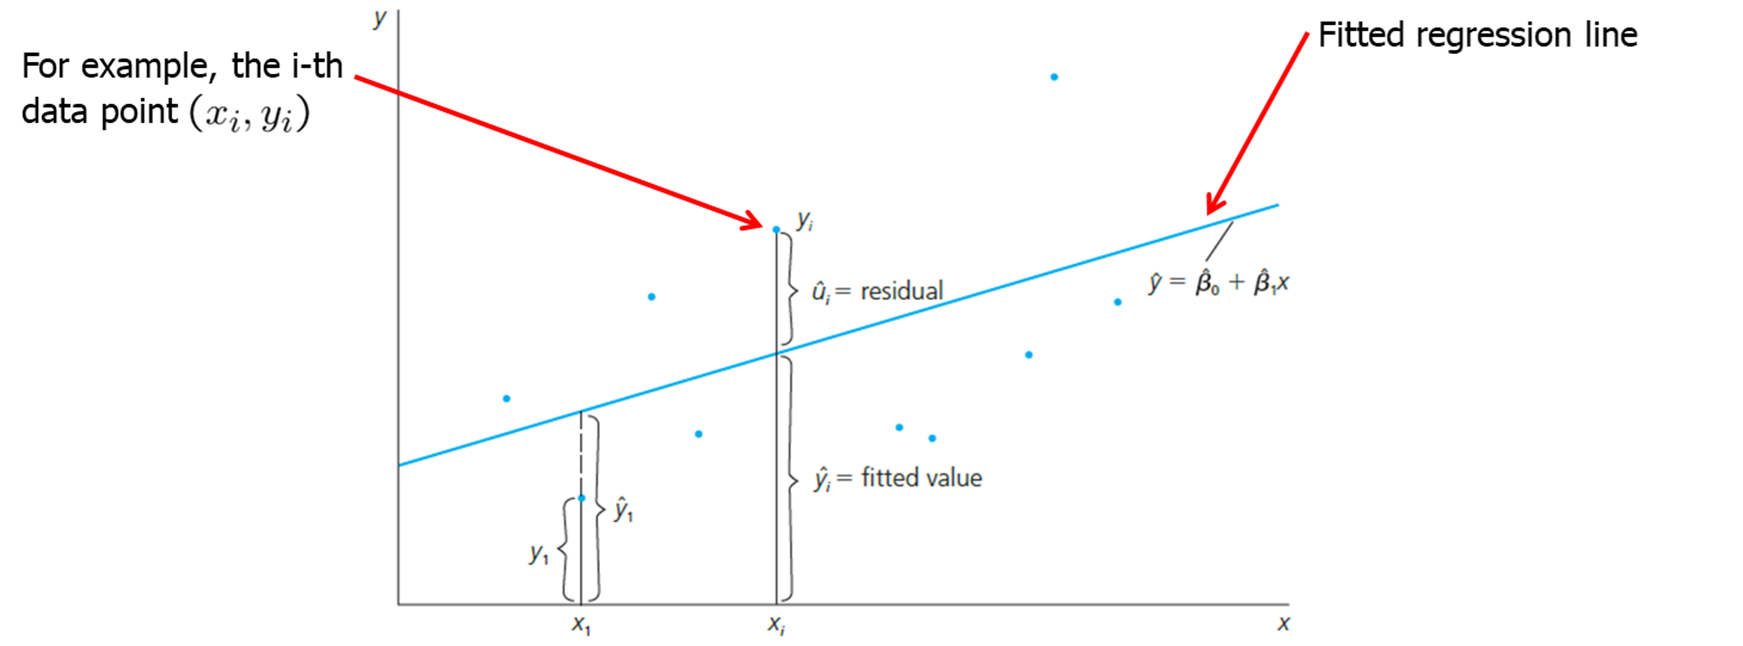
\includegraphics[width=1\linewidth]{figs/ols_fit.png}
\end{figure}


}


%%%%%%%%%%%%%%%%%%%%%%%%%%%%%%%%%%


\frame<beamer>{\frametitle{\textcolor{CUNEFOrange}{ 
Example of a simple regression
 }}

 \begin{itemize}
     \item CEO salary and return on equity


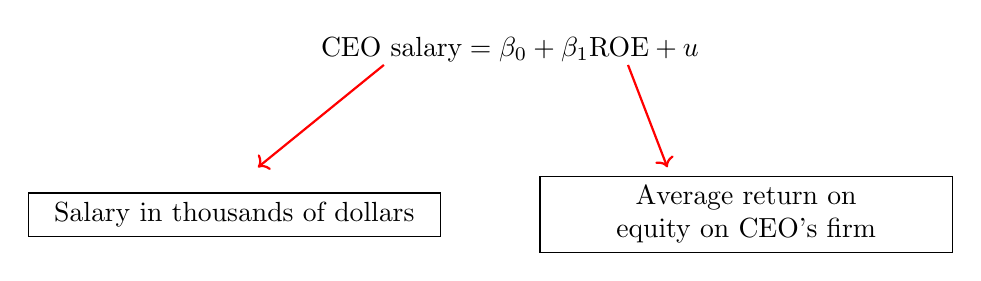
\begin{tikzpicture}

    % Equation
    \node at (0, 0) {\( \text{CEO salary} = \beta_0 + \beta_1 \text{ROE} + u \)};

    % Annotation for y (Dependent variable)
    \node[draw, rectangle, text width=5cm, align=center] at (-3.5, -2.1) {Salary in thousands of dollars};
    \draw[->, red, thick] (-1.6,-0.2) -- (-3.2,-1.5);


    % Annotation for x (Independent variable)
    \node[draw, rectangle, text width=5cm, align=center] at (3, -2.1) {Average return on\\ equity on CEO's firm};
    \draw[->, red, thick] (1.5,-0.2) -- (2,-1.5);


\end{tikzpicture}

\item Fitted regression:
$$
\widehat{\text {CEO salary}}=963.191+18.501 \text {ROE}
$$
If the return on equity increases by 1 percent, then salary is predicted to change by $\$ 18,501$


 \end{itemize}

}


%%%%%%%%%%%%%%%%%%%%%%%%%%%%%


\frame<beamer>{\frametitle{\textcolor{CUNEFOrange}{ 
Example of a simple regression }}


\begin{columns}
\column{.6\textwidth}
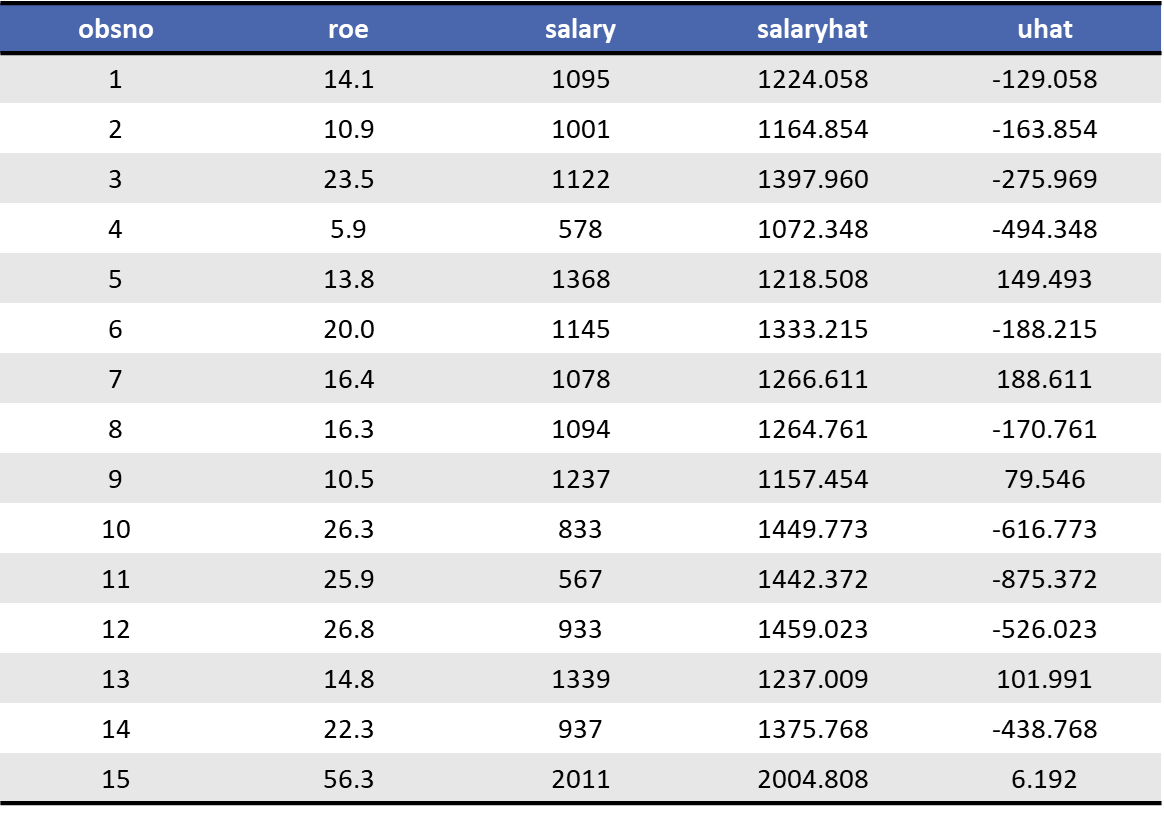
\includegraphics[width=1\linewidth]{figs/salary.png}
\column{.4\textwidth}
\begin{itemize}
\item  This table presents fitted values and residuals for 15 CEOs.\medskip
\item  For example, the $12^{\text {th }}$ CEO's predicted salary is $\$ 526,023$ higher than their actual salary.\medskip
\item  By contrast the $5^{\text {th }}$ CEO's predicted salary is $\$ 149,493$ lower than their actual salary.
\end{itemize}
\end{columns}



}



%%%%%%%%%%%%%%%%%%%%%%%%%%%%%
\section{Goodness of fit}

\frame<beamer>{\frametitle{\textcolor{CUNEFOrange}{ 
Goodness of fit: How well does an explanatory variable explain the dependent variable?
 }}

\begin{itemize}
    \item \textbf{Total sum of squares}: represents total variation in the dependent variable
$$
SST \equiv \sum_{i=1}^n\left(y_i-\bar{y}\right)^2
$$

\item \textbf{Explained sum of squares}: represents variation explained by regression
$$
SSE \equiv \sum_{\substack{i=1}}^n\left(\hat{y}_i-\bar{y}\right)^2
$$

\item 

\textbf{Residual sum of squares}: represents variation not explained by regression
$$
SSR \equiv \sum_{i=1}^n \hat{u}_i{ }^2 
$$



\end{itemize}

}



%%%%%%%%%%%%%%%%%%%%%%%%%%%%%


\frame<beamer>{\frametitle{\textcolor{CUNEFOrange}{ 
Goodness of fit: How well does an explanatory variable explain the dependent variable?
 }}

\begin{itemize}

    \item Decomposition of total variation:
    $$    
    \text{Total variation (SST) = Explained part (SSE) + Unexplained part (SSR)}
    $$

    \item Goodness-of-fit measure (R-squared)
    $$
R^2 \equiv \frac{S S E}{S S T}=1-\frac{S S R}{S S T}
$$
R-squared measures the fraction of the total variation that is explained by the regression

\end{itemize}

}



%%%%%%%%%%%%%%%%%%%%%%%%%%%%%


\frame<beamer>{\frametitle{\textcolor{CUNEFOrange}{ 
Goodness of fit: How well does an explanatory variable explain the dependent variable? }}

\begin{itemize}

    \item CEO salary and return on equity
    $$
\begin{aligned}
& \widehat{\text {CEO salary }}=963.191+18.501 \text {ROE} \\
& n=209, \quad R^2=0.0132
\end{aligned}
$$
The regression explains only $1.3 \%$ of the total variation in salaries.


\end{itemize}


}



%%%%%%%%%%%%%%%%%%%%%%%%%%%%%

\section{Incorporating non-linearities}
\frame<beamer>{\frametitle{\textcolor{CUNEFOrange}{ 
Incorporating non-linearities: Semi-logarithmic form
 }}

\begin{itemize}
    \item Regression of log wages on years of education
    $$
\log (\text { wage })=\beta_0+\beta_1 e d u c+u
$$

\item This changes the interpretation of the regression coefficient:
$$
\beta_1=\frac{\Delta \log (\text { wage })}{\Delta \text { educ }}=\frac{1}{\text { wage }} \cdot \frac{\Delta \text { wage }}{\Delta \text { educ }}=\frac{\frac{\Delta \text { wage }}{\text { wage }}}{\Delta\text { educ }}
$$
Now $\beta_1$ measures the \textbf{percentage change of wage} if \textbf{years of education are increased by one year}.
\end{itemize}

}



%%%%%%%%%%%%%%%%%%%%%%%%%%%%%


\frame<beamer>{\frametitle{\textcolor{CUNEFOrange}{ 
Incorporating non-linearities: Semi-logarithmic form
 }}



\begin{columns}
\column{.4\textwidth}
\begin{itemize}
    \item Fitted regression:
    $$
\widehat{\log }(\text { wage })=0.584+0.083 \mathrm{educ}
$$
The wage increases by $8.3 \%$ for every additional year of education (= return to another year of education)
\end{itemize}\column{.6\textwidth}
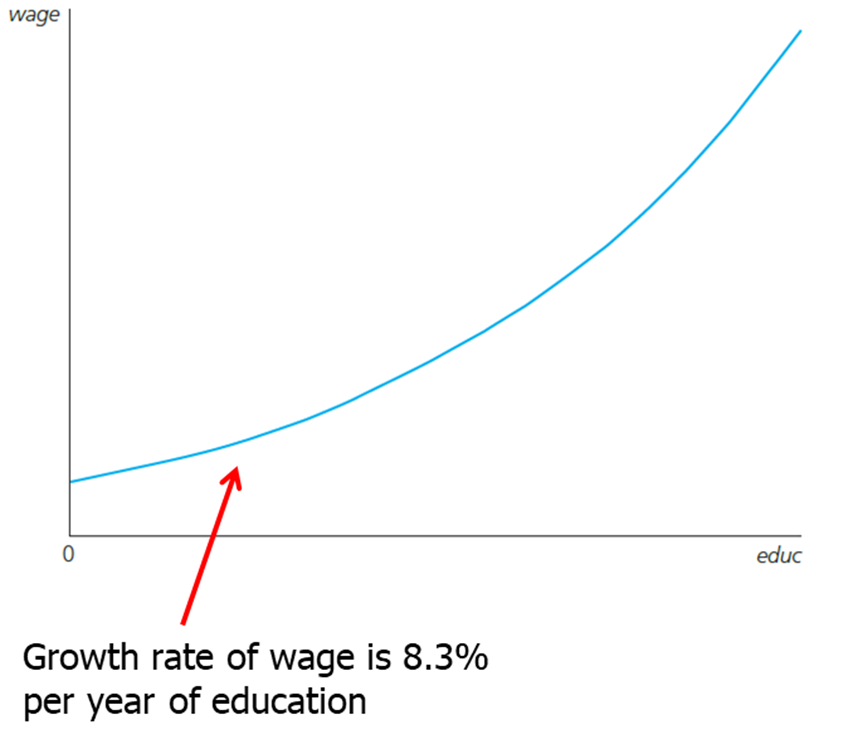
\includegraphics[width=0.8\linewidth]{figs/log_lin.png}
\end{columns}

}



%%%%%%%%%%%%%%%%%%%%%%%%%%%%%


\frame<beamer>{\frametitle{\textcolor{CUNEFOrange}{ 
Incorporating nonlinearities: Log-logarithmic form
 }}

\begin{itemize}
    \item Natural log of CEO salary and natural log of his/her firm sales:
$$
\log (\text { salary })=\beta_0+\beta_1 \log (\text { sales })+u
$$

\item This changes the interpretation of the regression coefficient:
    \[
    \beta_1 = \frac{\Delta \log (\text{salary})}{\Delta \log (\text{sales})} = \frac{\frac{\Delta \text{salary}}{\text{salary}}}{\frac{\Delta \text{sales}}{\text{sales}}}
    \]
    \begin{itemize}
        \item \textbf{Percentage} change in salary if sales increase by 1\%.
        \item Logarithmic changes are always percentage changes.
    \end{itemize}
\end{itemize}


}




%%%%%%%%%%%%%%%%%%%%%%%%%%%%%


\frame<beamer>{\frametitle{\textcolor{CUNEFOrange}{ 
Incorporating nonlinearities: Log-logarithmic form }}

\begin{itemize}
    \item CEO salary and firm sales: fitted regression
    \[
    \widehat{\log(\text{salary})} = 4.822 + 0.257 \log(\text{sales})
    \]
    \begin{itemize}
        \item \(+1\%\) sales \(\rightarrow\) \(+0.257\%\) salary
    \end{itemize}
\end{itemize}

}



%%%%%%%%%%%%%%%%%%%%%%%%%%%%%

\section{Expected values and variances of the OLS estimators}
\frame<beamer>{\frametitle{\textcolor{CUNEFOrange}{ 
Expected values and variances of the OLS estimators
 }}

\begin{itemize}
    \item The estimated regression coefficients are \textbf{random variables} because they are calculated from a \textbf{random sample}
$$
\widehat{\beta}_1=\frac{\sum_{i=1}^n\left(x_i-\bar{x}\right)\left(y_i-\bar{y}\right)}{\sum_{i=1}^n\left(x_i-\bar{x}\right)^2}, \quad \widehat{\beta}_0=\bar{y}-\widehat{\beta}_1 \bar{x}
$$
Data is random and depends on particular sample that has been drawn

\item The question is:  What the estimators will estimate on average and how large will their variability be in repeated samples
$$
E\left(\widehat{\beta}_0\right)=?, E\left(\widehat{\beta}_1\right)=? \quad \operatorname{Var}\left(\widehat{\beta}_0\right)=?, \operatorname{Var}\left(\widehat{\beta}_1\right)=?
$$

\end{itemize}
}

%%%%%%%%%%%%%%%%%%%%%%%%%%%%%


\frame<beamer>{\frametitle{\textcolor{CUNEFOrange}{ 
Standard assumptions for the linear regression model
 }}

\begin{itemize}
    \item Assumption SLR. 1 (Linear in parameters)

$$
y=\beta_0+\beta_1 x+u \longleftarrow \begin{aligned}
& \text { In the population, the relationship } \\
& \text { between } \mathrm{y} \text { and } \mathrm{x} \text { is linear }
\end{aligned}
$$

\item  Assumption SLR. 2 (Random sampling)

$$
\left\{\left(x_i, y_i\right): i=1, \ldots, n\right\} \longleftarrow \begin{aligned}
& \text { The data is a random sample } \\
& \text { drawn from the population }
\end{aligned}
$$
\medskip
$$
y_i=\beta_0+\beta_1 x_i+u_i \longleftarrow \begin{aligned}
& \text { Each data point therefore follows } \\
& \text { the population equation }
\end{aligned}
$$

\end{itemize}
}


%%%%%%%%%%%%%%%%%%%%%%%%%%%%%


\frame<beamer>{\frametitle{\textcolor{CUNEFOrange}{ 
Standard assumptions for the linear regression model
 }}

\begin{itemize}
    \item Assumption SLR. 3 (Sample variation in the explanatory variable)
$$
\sum_{i=1}^n\left(x_i-\bar{x}\right)^2>0
$$
The values of the explanatory variables are not all the same (otherwise it would be impossible to study how different values of the explanatory variable lead to different values of the dependent variable)

\item Assumption SLR. 4 (Zero conditional mean)
$$
E\left(u_i \mid x_i\right)=0
$$
The value of the explanatory variable must contain no information about the mean of the unobserved factors
\end{itemize}

}


%%%%%%%%%%%%%%%%%%%%%%%%%%%%%

\frame<beamer>{\frametitle{\textcolor{CUNEFOrange}{ 
Unbiasedness of OLS }}

\begin{itemize}
    \item Under assumptions SLR1 -- SLR4, we can show that:
    $$
E\left(\widehat{\beta}_0\right)=\beta_0, E\left(\widehat{\beta}_1\right)=\beta_1
$$


\item Interpretation of unbiasedness:
\begin{itemize}
    \item The estimated coefficients may be smaller or larger, depending on the sample that is the result of a random draw.
 \item However, on average, they will be equal to the values that characterize the true relationship between $y$ and $x$ in the population.
 \item ``On average'' means if sampling was repeated, i.e. if drawing the random sample and doing the estimation was repeated many times.
 \item In a given sample, estimates may differ considerably from true values.
\end{itemize}

\end{itemize}
}


%%%%%%%%%%%%%%%%%%%%%%%%%%%%%

\frame<beamer>{\frametitle{\textcolor{CUNEFOrange}{ 
Variances of the OLS estimators
 }}

\begin{itemize}
    \item Depending on the sample, the estimates will be nearer or farther away from the true population values.
\item How far can we expect our estimates to be away from the true population values on average (= sampling variability)?
\item Sampling variability is measured by the estimator's variances
$$
\operatorname{Var}\left(\widehat{\beta}_0\right), \operatorname{Var}\left(\widehat{\beta}_1\right)
$$

\item Assumption SLR. 5 (Homoskedasticity)
$$
\operatorname{Var}\left(u_i \mid x_i\right)=\sigma^2 \longleftarrow \begin{aligned}
& \text { The value of the explanatory variable must } \\
& \text { contain no information about the variability } \\
& \text { of the unobserved factors }
\end{aligned}
$$

\end{itemize}
}


%%%%%%%%%%%%%%%%%%%%%%%%%%%%%

\frame<beamer>{\frametitle{\textcolor{CUNEFOrange}{ 
Graphical illustration of homoskedasticity
 }}

\begin{figure}
    \centering
    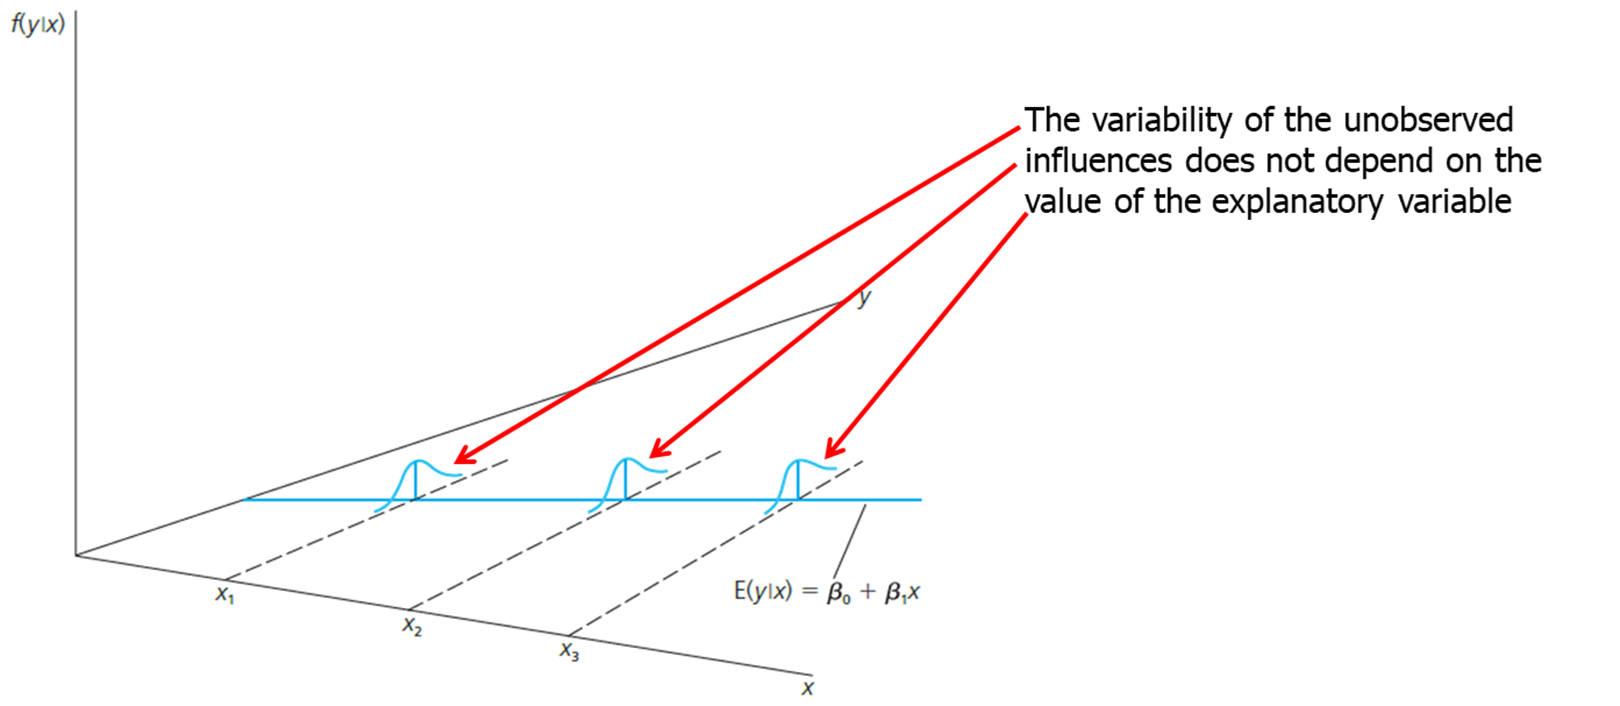
\includegraphics[width=1\linewidth]{figs/homosk.png}
\end{figure}

}


%%%%%%%%%%%%%%%%%%%%%%%%%%%%%

\frame<beamer>{\frametitle{\textcolor{CUNEFOrange}{ 
An example for heteroskedasticity: Wage and education
 }}

\begin{figure}
    \centering
    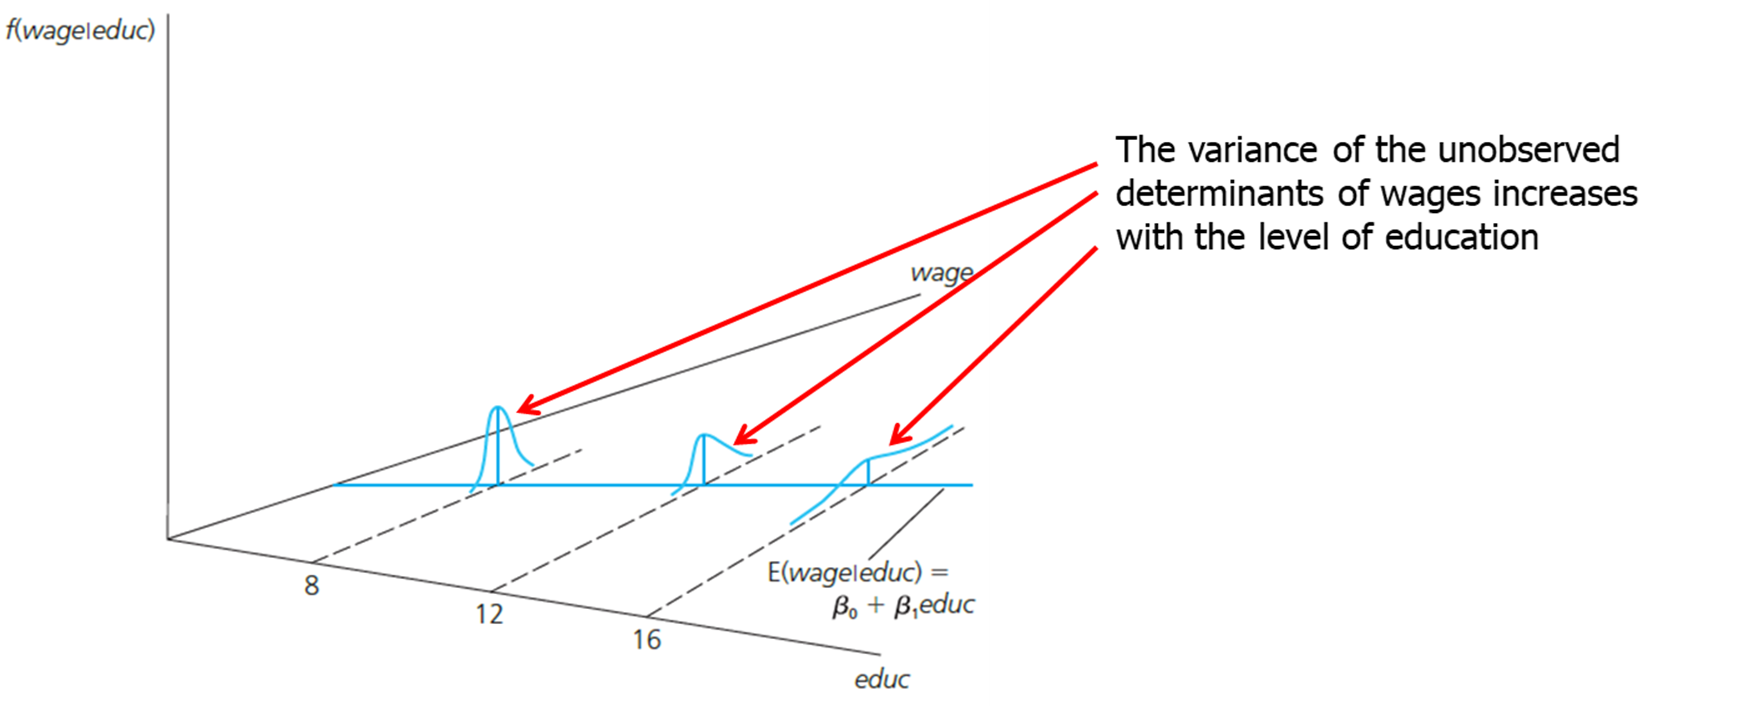
\includegraphics[width=1\linewidth]{figs/heterosk.png}
\end{figure}
}


%%%%%%%%%%%%%%%%%%%%%%%%%%%%%

\frame<beamer>{\frametitle{\textcolor{CUNEFOrange}{ 
Variances of the OLS estimators }}

\begin{itemize}
    \item Under assumptions SLR. 1 -- SLR.5:
$$
\begin{aligned}
& \operatorname{Var}\left(\widehat{\beta}_1\right)=\frac{\sigma^2}{\sum_{i=1}^n\left(x_i-\bar{x}\right)^2}=\frac{\sigma^2}{S S T_x} \\
& \operatorname{Var}\left(\widehat{\beta}_0\right)=\frac{\sigma^2 n^{-1} \sum_{i=1}^n x_i^2}{\sum_{i=1}^n\left(x_i-\bar{x}\right)^2}=\frac{\sigma^2 n^{-1} \sum_{i=1}^n x_i^2}{S S T_x}
\end{aligned}
$$

\item Conclusion: The sampling variability of the estimated regression coefficients will be the higher, the larger the variability of the unobserved factors, and the lower, the higher the variation in the explanatory variable.
\end{itemize}

}


%%%%%%%%%%%%%%%%%%%%%%%%%%%%%

\frame<beamer>{\frametitle{\textcolor{CUNEFOrange}{ 
Estimating the error variance
 }}

\begin{itemize}
    

\item $$
\operatorname{Var}\left(u_i \mid x_i\right)=\sigma^2=\operatorname{Var}\left(u_i\right) \longleftarrow \text { The variance of } \mathrm{u} \text { does not depend on } \mathrm{x} \text {, }
$$

\item $$
\hat{\sigma}^2=\frac{1}{n} \sum_{i=1}^n\left(\hat{u}_i-\overline{\hat{u}}_i\right)^2=\frac{1}{n} \sum_{i=1}^n \hat{u}_i^2 \quad \longleftarrow\begin{aligned}
& \text { One could estimate the variance of the } \\
& \text { errors by calculating the variance of the } \\
& \text { residuals in the sample; unfortunately } \\
& \text { this estimate would be biased }
\end{aligned}
$$

\item $$
\widehat{\sigma}^2=\frac{1}{n-2} \sum_{i=1}^n \widehat{u}_i^2 \longleftarrow \begin{aligned}
& \text { An unbiased estimate of the error variance can be obtained by } \\
& \text { substracting the number of estimated regression coefficients } \\
& \text { from the number of observations }
\end{aligned}
$$

\end{itemize}
}


%%%%%%%%%%%%%%%%%%%%%%%%%%%%%

\frame<beamer>{\frametitle{\textcolor{CUNEFOrange}{ 
Calculation of standard errors for regression coefficients
 }}

$$
\begin{aligned}
& \operatorname{se}\left(\widehat{\beta}_1\right)=\sqrt{\widehat{\operatorname{Var}}\left(\widehat{\beta}_1\right)}=\sqrt{\widehat{\sigma}^2 / S S T_x} \\[1cm]
& \operatorname{se}\left(\hat{\beta}_0\right)=\sqrt{\widehat{\operatorname{Var}}\left(\hat{\beta}_0\right)}=\sqrt{\hat{\sigma}^2 n^{-1} \sum_{i=1}^n x_i^2 / S S T_x}
\end{aligned}
$$

The estimated standard deviations of the regression coefficients are called ``standard errors.'' They measure how precisely the regression coefficients are estimated.


}


%%%%%%%%%%%%%%%%%%%%%%%%%%%%%
\section{Regression on a binary explanatory variable}
\frame<beamer>{\frametitle{\textcolor{CUNEFOrange}{ 
Regression on a binary explanatory variable
 }}

\begin{itemize}
    \item Suppose that $x$ is either equal to 0 or 1
$$
\begin{aligned}
& y=\beta_0+\beta_1 x+u \\
& E(y \mid x=0)=\beta_0 \quad E(y \mid x=1)=\beta_0+\beta_1
\end{aligned}
$$

\item  This regression allows the mean value of $y$ to differ depending on the state of x

$$
\beta_1=E(y \mid x=1)-E(y \mid x=0)
$$

\item Note that the statistical properties of OLS are no different when x is binary
\end{itemize}

}


%%%%%%%%%%%%%%%%%%%%%%%%%%%%%

\frame<beamer>{\frametitle{\textcolor{CUNEFOrange}{ 
Regression on a binary explanatory variable
 }}

\begin{itemize}
    \item Example: The effects of a job training program on earnings
    
\item Real earnings are regressed on a binary variable indicating participation in a job training program.
$$
\begin{aligned}
& \widehat{re78}=4.55+1.79 \text { train } \\
& n=445, R^2=0.018
\end{aligned}
$$
re78 is real earnings in 1978 measured in thousands of dollars. train is a binary variable equal to 1 if the individual participated in the job training program 

\item  Those who participated in the training program have earnings $\$ 1,790$ higher than those who did not participate.

\item This represents a $39.3 \%$ increase over the $\$ 4,550$ average earnings from those who did not participate.
\end{itemize}


}


%%%%%%%%%%%%%%%%%%%%%
% Back Page
%%%%%%%%%%%%%%%%%%%%
\NoLogoFootline
{\usebackgroundtemplate{%

\includegraphics[width=\paperwidth,height=\paperheight]{figs/back_page.png}}
\slide{}{}}

%%%%%%%%%%%%%%%%%%%%%%%%%%%%%

\end{document}